\documentclass{article}
\usepackage[utf8]{inputenc}
\usepackage{graphicx}

\title{Unsupervised Learning}
% Deep Learning Note for April 15
\author{Yunhao Li}
% Authors: Yunhao Li 04/15/19.

\begin{document}

\maketitle

\section{Theory}
21:45 - 51:55
\subsection{Introduction}

The term is "Unsupervised Learning" or "Self-supervised Learning". And "Self-supervised Leaning" maybe more descriptive of what is going on. \\ \\

The main motivation for Self-supervised Leaning is that it is kind of learning that takes place in human or animals. \\ \\

The main limitation of the learning system(AI and machine learning in particular) today is the fact that we are limited to use supervised learning or reinforcement learning. Both of them are very inefficient because they requires either many many trials or a lot of data manually annotated by humans. That limits information that we can feed the machine for it to learn. \\ \\

The idea of unsupervised learning is that the machine should discover the structure of the given data as much as possible. (e.g. Children learn new visual exception very quickly because they already have elaborated internal representations mostly by observation and a little by interaction.) \\ \\

How can we do it for machines? It has vary practical consequences. For example, Facebook want to translate every language to other languages. There are about 5k-7k languages. And we don't have parallel text translated from every language from others. So supervised learning doesn't work. People think about multi-lingual translator with encoder that encode text in each language into some internal representation of the meaning of the sentence and separate decoders for every language. So the problem of learning $n^2$ translator is transformed into $n$ encodes and $n$ decodes. Even so, the significant amount of training data is needed. \\ \\    

One thing that really works very well for reducing needed labeled samples to train for particular task is transfer learning. For example, in vision, you train a gigantic ConvNet on enormous amounts of data that either have been manually labeled or you train it to predict labels of free data(e.g. photos on Instagram). Then you chopped of the last layer of the network and you use the representation learned this way as input to supervised classifier for particular task. \\ \\

There is a lot of situation that we don't have a lot of labeled data. People want to detect rare occurrences of things. There is an example: The gunshot murderer of New Zealand broadcast the video live on Facebook. And the automatic video classification system didn't detected that video should be shut down. The problem is that, firstly we don't have many training samples. How do you train machine with very few samples? The similar problem in medicine is much more positive application where you want to train a system to detect rare diseases in medical images or things like that.\\ \\

So how do get machines to learn with very small amount of data? Here is another much more immediate example: Many companies try to develop automatic driving systems. It is very hard because perception systems need to be trained with lots of cases, which maybe very rare actually. You'd like machine to have some common sense to realize some situations. There is an example of Tesla. There is a white truck stuck across the road, and the radar didn't see that stationary object. The radar did detect stationary things but it eliminated it as an obstacle. They only sees cars moving around you or next to you. The vision that Tesla used is a convolution net. And it is not trained with this situation(white truck). So it assumed the road is open because the view is white and it didn't break.\\ \\

Here is another issue: how do human learns to drive a car after training for about 20 hours? If you try to use a existing reinforcement learning method to train a car to drive itself, you will have to do it in a simulator. Because the system will learns from many thousands of accidents and it will learns not to do the wrong decision. It just tries something and sees what the result is. And the better things may happen next time. Human have a pretty good model that predicts what may happen. So we can know the result without trying it. This model is acquired by observing which is a form of unsupervised learning.\\ \\
So that is a big obstacle to progress in AI is the fact we don't now entirely how to use unsupervised learning in a good way. Another one is that we need to combine deep learning with reasoning. We need to train systems to reason, not just perceive. \\ \\

The reason we need unsupervised learning is the fact that the number of the amount of the data we ask machine to predict is sort of different. These different paradigms of learning are very different. \\ \\

In the reinforcement learning, you ask machine to predict a reward(cost) of a particular sequence of action. The system just gets a reward instead of much information in the end. 
It is a very sparse feedback, which means the number of trials needed is very large because in every trial you only give it a little information. \\ \\

In supervised learning, you give 10-10,000 bits per sample. When doing ImageNet classification, for example, there is 1 thousands categories. The information is 10 bits. \\ \\

Think about this situation: you showed machine with video clips and ask it to predict what happened next. And you show it what happens. The information you give to machine is much larger(10 frames have really huge amounts information for machine to predict). So if it is able to make that prediction, it has to learn a lot about the structure of the wild. For example: if you are a learning machine and your entire world consist of short video clips. And the camera transfers a little bit to the left or right(The data also includes how much the camera moves). We want to train the machine to predict what it looks like after the move. If the machine can learn it, it has to learn internally some representation of depth. So train a machine to make that prediction will implicitly have it learn: 
\begin{enumerate}
    \item The world of 3D dimension. 
    \item Raise depth for everything
    \item Predict depth from a single(or several) image.
\end{enumerate} 
After it predicts, something pops up like occlusion edges. The edges will move after moving the view.\\ \\

Through the prediction based learning, the machine will learn a lot such as 3D world and the objects in the world separated from the background unsupervisedly. And because you are asking a lot from machine, so it learns a lot of regularities of the world with relatively small number of samples. \\ \\

There is a analogy of machine learning and the cake. Almost everything we learn we learned in unsupervised learning. We learn a little bit through supervised learning, and we learn a tiny bit through reinforcement learning. \\
\begin{figure}[ht]
\centering
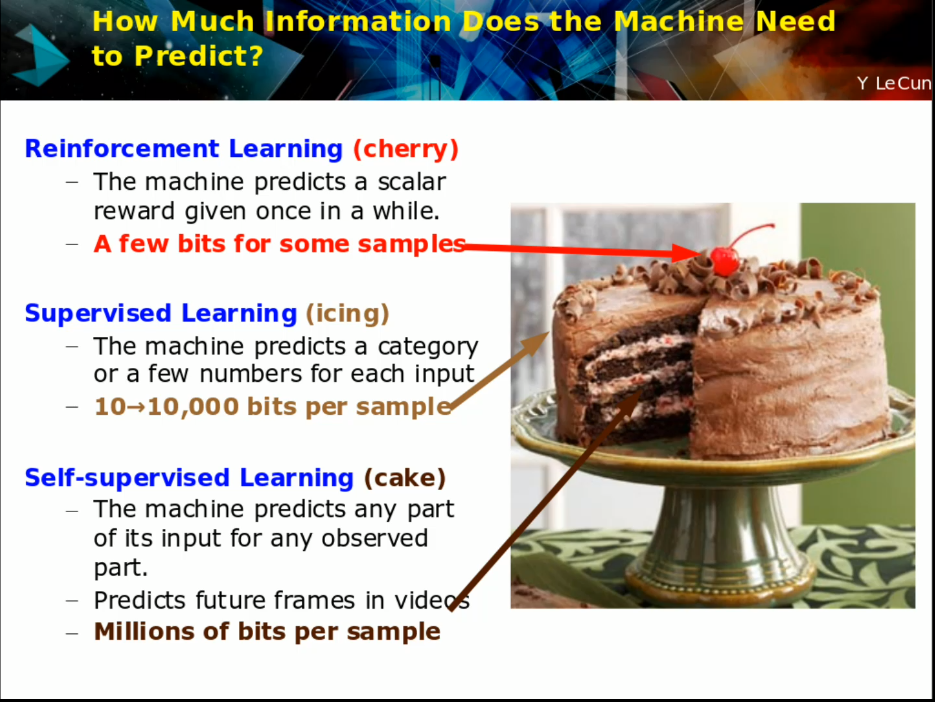
\includegraphics[scale=0.6]{cake.png}
\caption{Cake analogy}
\label{fig:label}
\end{figure}
\\

Unsupervised learning seems succeeds in Natural Language Processing(NLP). The default best way to train a NLP system is to train an autoencoder or denoising autoencoder. The idea of BERT, you take a window of a dozen words over corpus. You take out about 15 percent of the words and you ask the system to predict what words are missing. It is type of autoencoder or denoising autoencoder in particular. After you going through billions of windows over text, you use the internal of this network as an input to a supervised task(text classification, summary, etc). That works really well. But that way does not perfectly worked in image recognition in video. \\ \\

Unsupervised learning is the dark matter of AI.
\begin{figure}[ht]
\centering
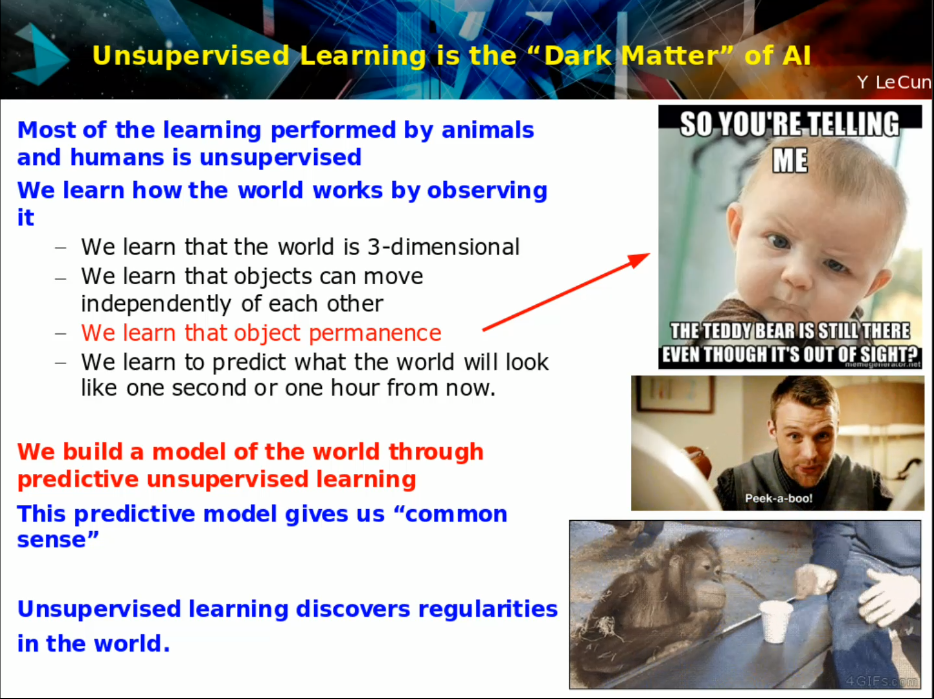
\includegraphics[scale=0.6]{DarkMatter.png}
\caption{Dark Matter. The cup trick.}
\label{fig2:label}
\end{figure}

The baby only learn the very elementary things and doesn't have the idea of the object permanence. If we take an object and hide it, and the baby doesn't know that it still exists. \\ \\

World model has many built-in knowledge, which is what we called common sense(usual, not the term). You can infer a lot from the few words, such as, it is a man, it is at work. And You can imagine the scenario. You know a lot because You know the constraints of the world. When our idea of the world is violated, there will be several attitudes. The first one is you pay attention because something you didn't predict actually occurred. That could be dangerous or funny. The reason you pay attention because you can learn something that violated your model and that means your model is wrong.\\ \\

How do we do unsupervised learning? \\ 
Prediction is kind of a reconstruction. For example, you can train a system to predict the end of a video from the beginning. But you can also do it in the other direction(given the end, predict what happened before). Completing the missing information, filling the blanks, that's the purpose of unsupervised learning.\\ \\

So there is a problem: if I ask you to predict the future of a video with given video clips, many plausible things can happen. There is no single correct answer for this. The energy base learning will be useful. We need to construct a predictor that can predict multiple things, not just one single future prediction. The world is not entirely predictable. There is a lot of uncertainty. The question is, how do construct machine to predict things. The immediate answer is we can predict a distribution instead of predicting a single point.(e.g. Put a pen on table and let it go. The pen falls in a different direction every time. The directions is in a distribution) If you want to predict a frame of video, there is a distribution of images. You will have to parameterize the distribution of images. The basic possible to parameterize the distribution. We don't have density models or condition models of natural images. The main issue is that we don't know how to represent normalized distributions. Giving a quality of goodness or badness to a particular image is maybe possible, but training this into a distribution is very hard. That is one reason for introducing energy base models.


\end{document}
